



\begin{frame}{\citetitle{MarcoNuno_Revista_2020_10_00} \footnotemark (1)}

\begin{columns}
\begin{column}{0.5\textwidth}
	\begin{itemize}
\item Es necesario herramientas para educar a pacientes con Diabetes para manejar su enfermedad.
\item Se propone una aplicación móvil que permita generar una simulación del comportamiento de la glucosa en un organismo con Diabetes a partir de modelos:
	\begin{itemize}
		\item Dosificación de insulina
		\item Ejercicio
		\item Ingesta de alimentos
	\end{itemize}
	\end{itemize}
\end{column}
\begin{column}{0.5\textwidth}
\begin{center}
     %%%%% this is a minipage, so \textwidth is already adjusted to the size of the column
     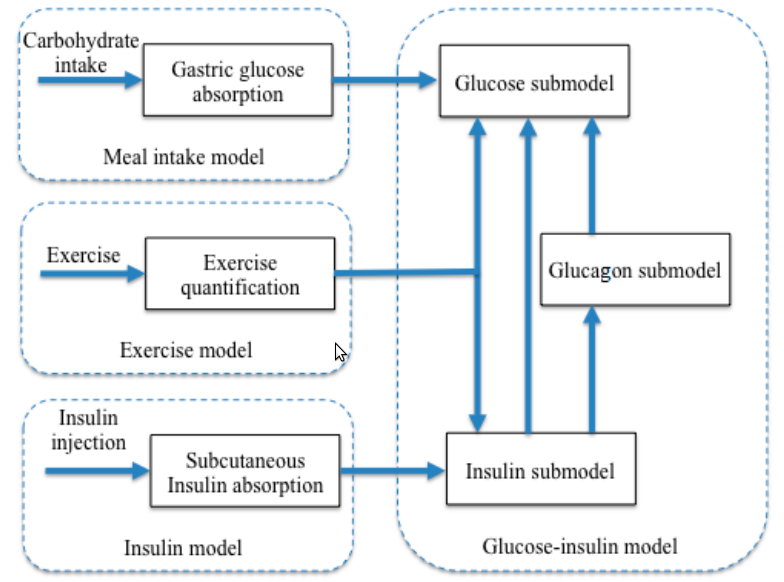
\includegraphics[width=0.99\textwidth]{Figs/Diabetes1}
     \end{center}
\end{column}
\end{columns}
\footnotetext[1]{\fullcite{MarcoNuno_Revista_2020_10_00}}
\setcounter{footnote}{0}
\end{frame}

\begin{frame}{\citetitle{MarcoNuno_Revista_2020_10_00} (2)}
\begin{columns}
\begin{column}{0.65\textwidth}
Pantallas de la aplicación:
	\begin{enumerate}
\item Pantalla inicial
\item Configuración de ingesta de alimentos
\item Configuración de dosificación de insulina
\item Configuración de configuración de rutina de ejercicio
\item Inicio de simulación
	\end{enumerate}
\end{column}
\begin{column}{0.40\textwidth}
\begin{center}
     %%%%% this is a minipage, so \textwidth is already adjusted to the size of the column
     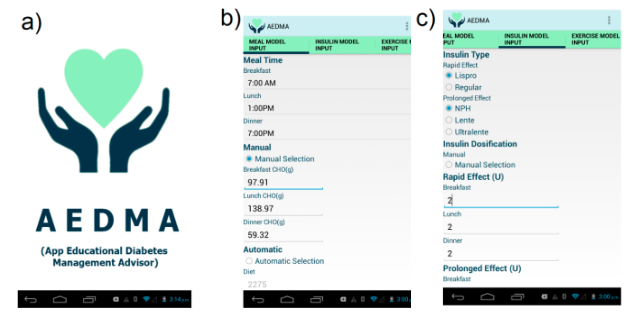
\includegraphics[width=0.99\textwidth]{Figs/Diabetes3}
     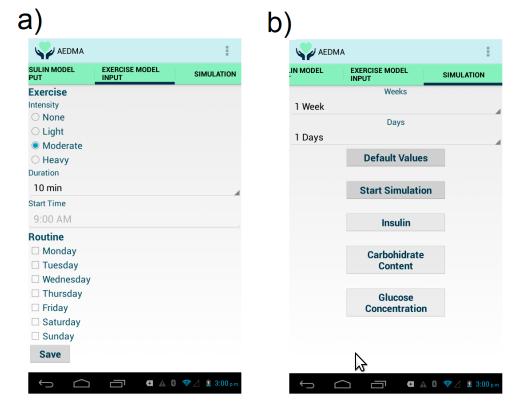
\includegraphics[width=0.66\textwidth]{Figs/Diabetes4}
     \end{center}
\end{column}
\end{columns}
\end{frame}

\begin{frame}{\citetitle{MarcoNuno_Revista_2020_10_00} (3) } 
\begin{columns}
\begin{column}{0.65\textwidth}
La aplicación genera una gráfica de comportamiento de la glucosa a lo largo del tiempo de simulación. Se muestran las gráficas para cuatro casos:
	\begin{itemize}
\item Pacientes controlados en cuanto a los niveles de glucosa (a y b)
\item Pacientes fuera de control debido a la falta de ejercicio y al exceso de carbohidratos (c y d)
	\end{itemize}
\end{column}
\begin{column}{0.35\textwidth}
\begin{center}
     %%%%% this is a minipage, so \textwidth is already adjusted to the size of the column
     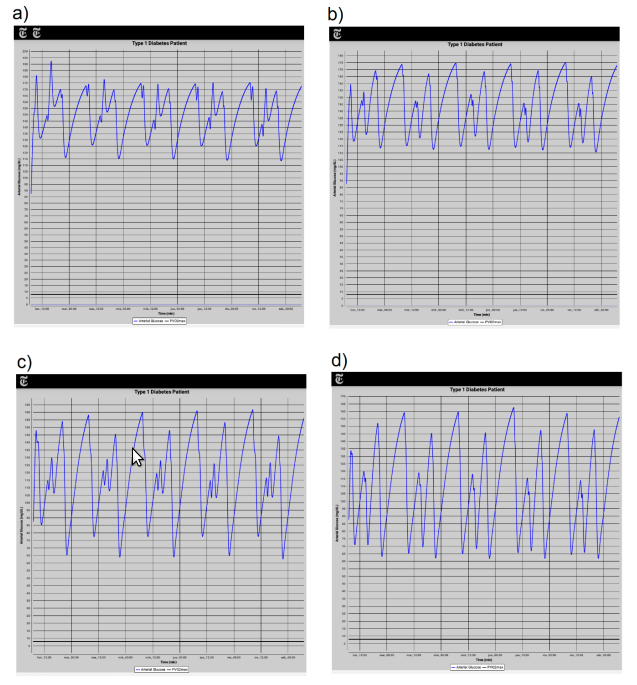
\includegraphics[width=0.99\textwidth]{Figs/Diabetes5}
     \end{center}
\end{column}
\end{columns}
\end{frame}



